\subsection{Content}

Software development projects, scientific researches and teaching computing science are difficult to organise, document and present. Reviewing a piece of code or publishing it has always required explanation and so far it has been recorded as a comment in the code or as a text file. This method of reporting analysis and algorithms is ineffective for the productivity and concentration of project's developers. 

Python is a programming language that is known as an easy to learn, code and prominent for data analysis, except that it has an inconvenient shell. Running, testing, debugging and documenting Python scripts has required the usage of various software tools, such as the command prompt (or another command-line interpreters), text editors and others. 

To overcome this drawback of Python, IPython has been created as a software tool, interactive shell for standard scientific Python scripts, that allows combination of styled text, code and data visualizations. It is designed to stimulate the writing, testing and debugging of Python code and it has a productive environment for analytical computing. \cite{mckinney2012python} Running Python scripts is effective for immediate response, since developers can see the results right away.

The \textit{IPython Observatory} project is exploring an explicit environment of researches available for everyone - e.g. open source repositories. GitHub,  web-based Git repository hosting service, is one of the most crucial web-sites as a source of information  on the Internet.\cite{gitHubWiki} A huge number of researchers have started to investigate and anlayze GitHub repostories so that they can understand how users are exploiting the site for collaboration on software. \cite{kalliamvakou2007promises} In order to assess the value of IPython in researches, the project is analyzing through the questions: how IPython is used in repositories? why should we consider investigating version control environments, such as GitHub or BitBucket, for scientific IPython notebooks? 

\subsection{Problem Statement}
\label{subsec:problem}

Normally, theoretical and experimental practices are representing two main aspects in the process of a research. Recently, computing is appearing to be one more important part of science. It is not only closely connected to theory and experiment, but it also has common features with them. Scientific programming is a crucial element of research analysis, since it gives faster and more accurate results - all calculations, models and visualizations can be computed with the help of software tools. As a consequence, scientific programming can be viewed as a another section of conducting researches.\cite{johansson2014introduction} However, how software is used in science and what are the problems that researchers encountered when using software?

Computational sciences bring great help and support to the field of journals and exploration, but together with that they have downsides - programming scripts need to be created for a specific area of study, which needs knowledge of both software implementation and the science of the investigated field. Usually analysts are well familiar with only the science that he is doing the research and as a consequence of that, s/he needs to gain computer programming skills. However, programming languages are challenging to learn and a lot of time and practicing is needed for the implementation of the functionality. The analysts might not have the necessary preparation and training in order to create the computations.  

Furthermore, the target readers would probably not be acquainted with the code in the research, so a proper documentation of the software scripts is required. Thoughts, ideas and findings also demand to be recorded for analysis and investigation of the gathered information. Researchers have discover an effective approach for detailing each aspect of a project - handwritten notebooks. They are mainly used for laboratory experiments. However, researchers have encountered problems with the usage of notebooks - they might not be well organised; each scientist has different style of writing and the reader might have difficulty of reading the notebook; tracking and predicting data with the handwritten notebook is challenging and time-consuming process;

The above problems show that scientists are striving to achieve in reproducible research\textit{" the ability of an entire experiment or study to be duplicated, either by the same researcher or by someone else working independently"}, and replication of results - \textit{"is the repetition of an experimental condition so that the variability associated with the phenomenon can be estimated"}. \cite{reproducibilityWiki} \cite{replicationWiki} They want to be able to produce more shareable document that would give details about the implemented code and the analysis of the findings at the same time. 

IPython Notebook is an open-source projects and they have become an option for scientific researches. The easy set-up and usability is allowing scientists, from different areas of study, to operate with it. It is worth investigating IPython usage in science, since it is an electronic version of the notebooks that researchers have. Also, the main feature of IPython, combining text, code and code output in one file, is of great interest for structuring scientists' ideas and computations. In order to assess the effectiveness of IPython in researches, we have to analyze how is it applied by them and what impact will it have on the problems mentioned above, the issues encountered with the usage of scientific software. 

As a consequence of that, there are specific features of software usage that the project needs to investigate in order to give effective assessment of IPython notebook - e.g. how many GitHub repositories are using IPython for scientific researches, how is it used in a specific area of study, depending on the text and code implemented, and others. These questions are illustrating challenges that the project has to confront in order to find the best approach of evaluation of the IPython notebook.  

\subsection{Proposed Approach}

The project has is analyzing in detail the IPython results from the GitHub search. GitHub is a widely used open source hosting service for projects and, recently, it has become effective place for sharing various researches and contributing to them. It has been chosen for investigation, since it allows tracking of data changes, commits, contributions and documentation. 

The analysis of IPython notebooks on GitHub is broken down to several steps, which are explained in more detail in section \ref{workplan}. Replication and reproducibility of IPython in researches will be the main elements of investigation - they are fundamental for replicating of scientific results. Furthermore, GitHub repositories are important part of projects, as well. The \textit{"The Promises and Perils of Mining GitHub"} is investigating possible threats to the validity of researches involving software projects hosted on GitHub.\cite{kalliamvakoupromises} Figure \ref{fig:github} is showing the results of the paper. 

\begin{figure}
\centering
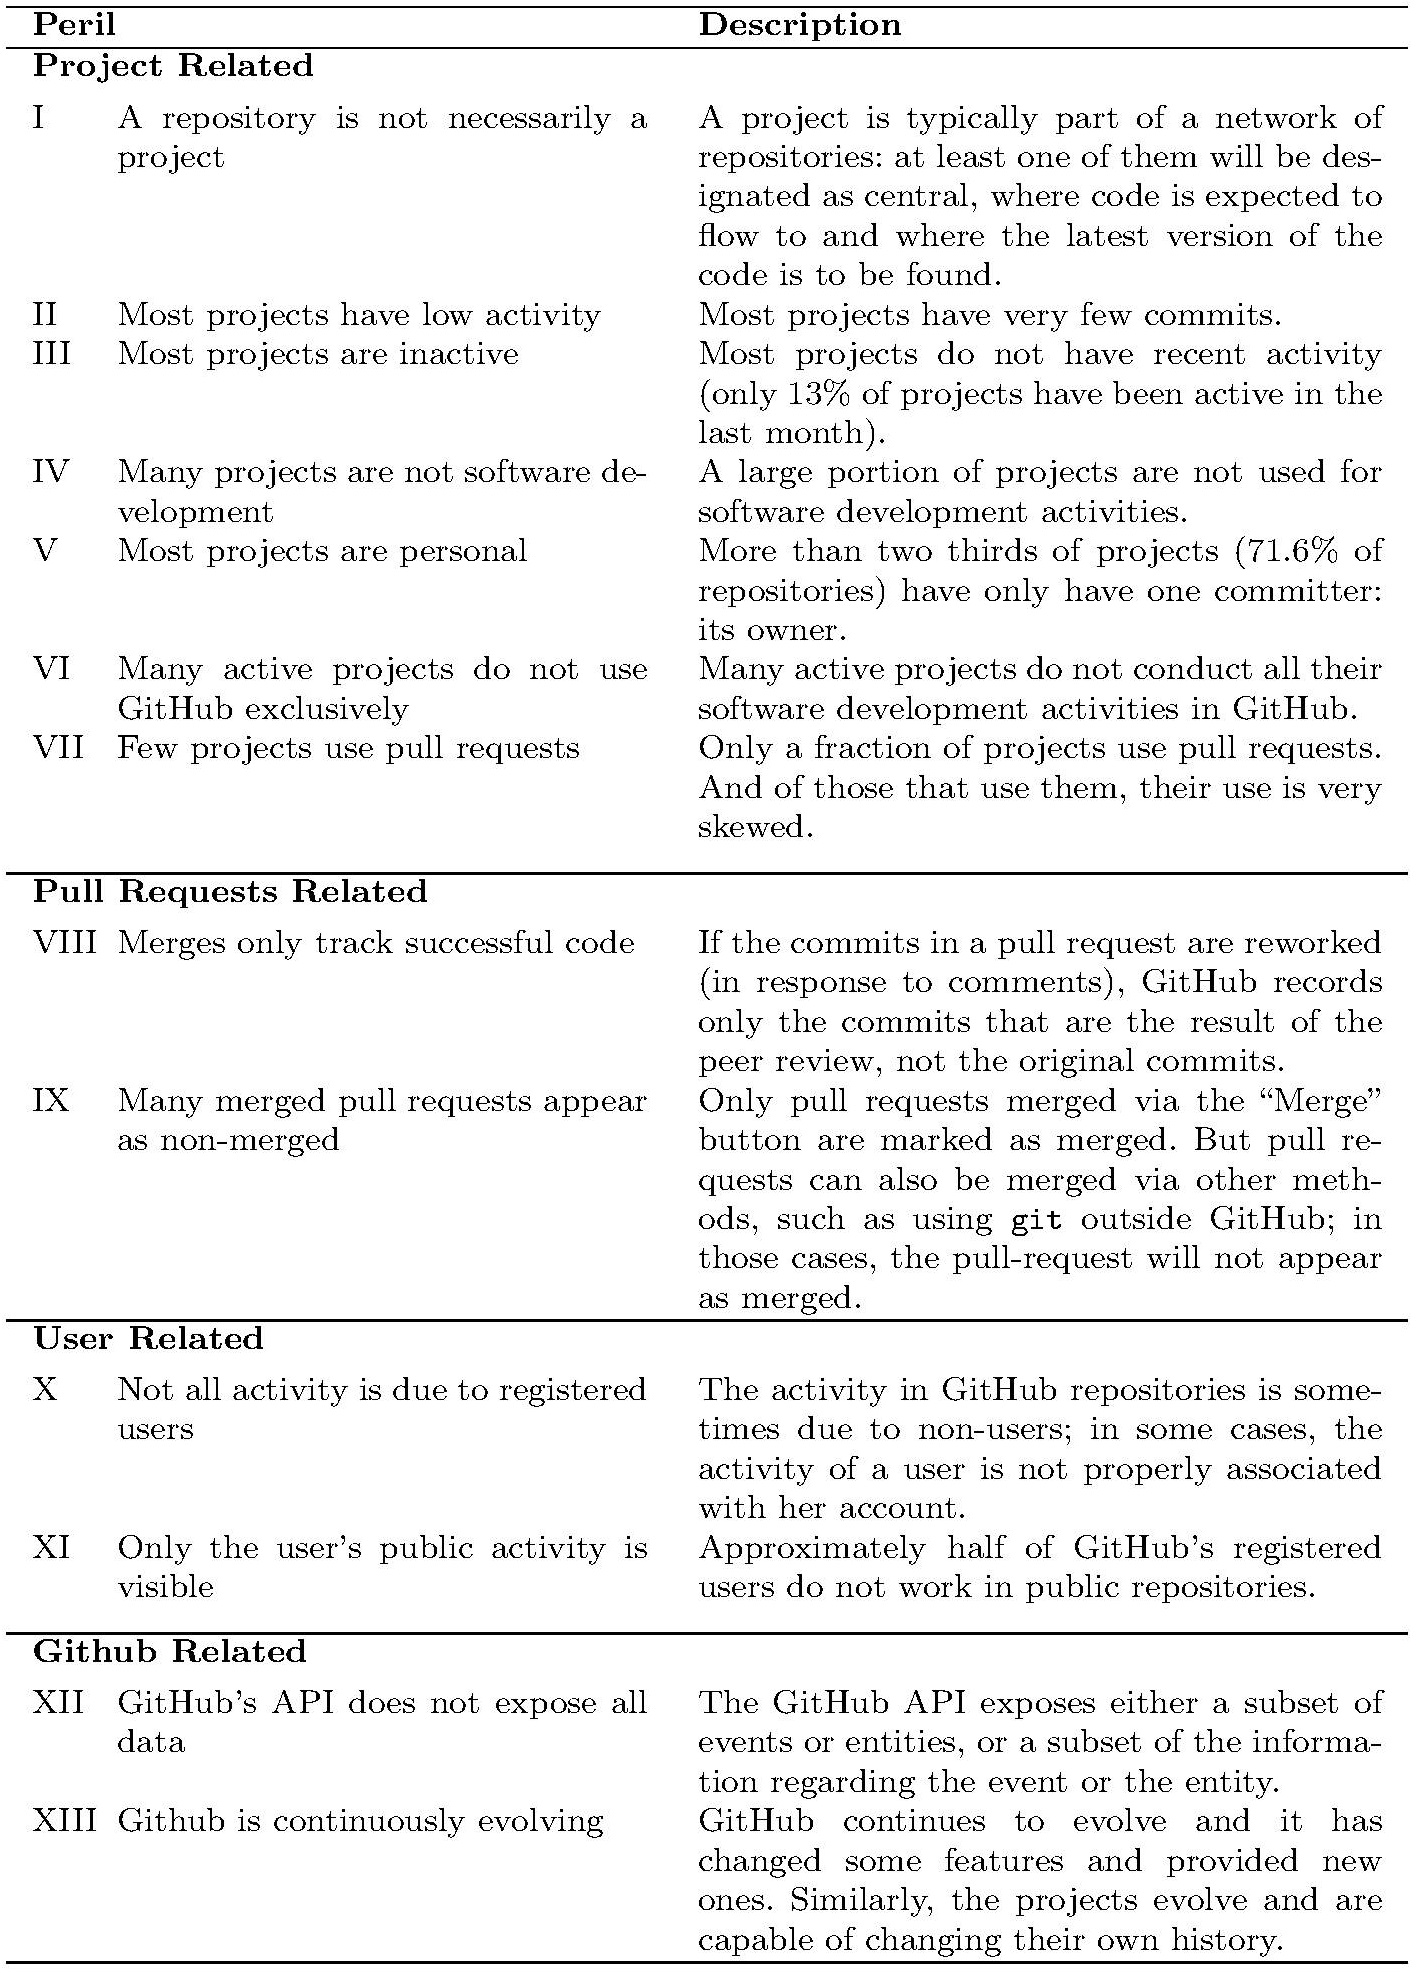
\includegraphics[scale=1.0]{images/file-page1}
\caption{The Promises and Perils of Mining GitHub Results}
\label{fig:github}
\end{figure}


\subsection{Structure of the paper}